\documentclass[UTF8]{ctexbook}
\usepackage{polyglossia}
\usepackage{tipa}
\usepackage{multicol}
\usepackage{multirow} 
\usepackage{mdframed}
\usepackage{longtable}

\usepackage{enumitem} %阿语字体有时缺itemize引导符的字形
\usepackage{wrapfig} % 环绕图片的正文内容

\usepackage{color}
\usepackage{graphicx}

\usepackage{tikz}
\usetikzlibrary{3d, arrows.meta} % 屈折变化太多了,不用3D真不行

\setotherlanguages{arabic}
\setotherlanguages{english}
\setotherlanguages{mongolian}

\newfontfamily\arabicfont[
    Script=Arabic, 
    BoldFont=KufiStandardGK, 
    ItalicFont=NotoNaskhArabic-Regular,
    Scale=1.2]
    {MicrosoftSansSerif}

\newfontfamily\mongolianfont[
    Script=Mongolian,
    Scale=1.3
]{AbkaiXanyan}

%% 自己的感悟笔记
\newenvironment{note}{
    \itshape
    \setlength{\parindent}{0pt}
    \begin{mdframed}[linewidth=0pt, backgroundcolor=gray!15]
}{
    \end{mdframed}
}

%% 课上的强调
\newenvironment{attention}{
    \itshape
    \setlength{\parindent}{0pt}
    \begin{mdframed}[
        leftline=true,
        rightline=false,
        topline=false,
        bottomline=false,
        linecolor=gray!50,
        linewidth=3pt
    ]
}{
    \end{mdframed}
}

%%% 双语支持
\newcommand{\arm}[1]{\textarabic{#1}} % 正文中夹杂阿语
\newcommand{\ait}[1]{\itshape #1}
\newcommand{\abf}[1]{\bfseries #1}
\newcommand{\crm}[1]{\textenglish{#1}} % 阿语环境中夹杂中文
\newcommand{\ac}[2]{#2 \hspace*{0pt} \dotfill \hspace*{0pt} \arm{#1}} % 双语对照

%%% 辅助显示
% 表示变化方向的箭头,有两种方向
\newcommand{\cto}{$\rightarrow $ }
\newcommand{\ato}{$\leftarrow $ }
\newcommand{\tto}{%
    \iflanguage{arabic}{\ato}{\cto}%
}

\newcommand{\lecon}[1]{\fbox{P#1}} % 对应视频课程P数

\newcommand{\blue}[1]{\textcolor{blue}{#1}}
\newcommand{\red}[1]{\textcolor{red}{#1}}

\title{
    \arm{\abf{\Huge اَللُّغَةُ الْعَرَبِيَّةُ}} \\ \textbf{阿拉伯语笔记\\
    \normalsize 基于{\tiny(已经跑路的)}万门大学《阿拉伯语初级(上)》课程整理}
    \vfill}
\author{
    主讲教师:白\quad 野(\arm{مَنْصُورٌ})}
\date{\today}
\begin{document}
\maketitle

\chapter*{前言}

\vfill
\begin{center}

    \arm{\ait {\Large اُطْلُبُوْا العِلْمَ وَلَوْ في الصِّينِ.}}
    
    ~\\

    \emph{求知,哪怕在中国。}
\end{center}
\vfill

\begin{center}
    \begin{center}
        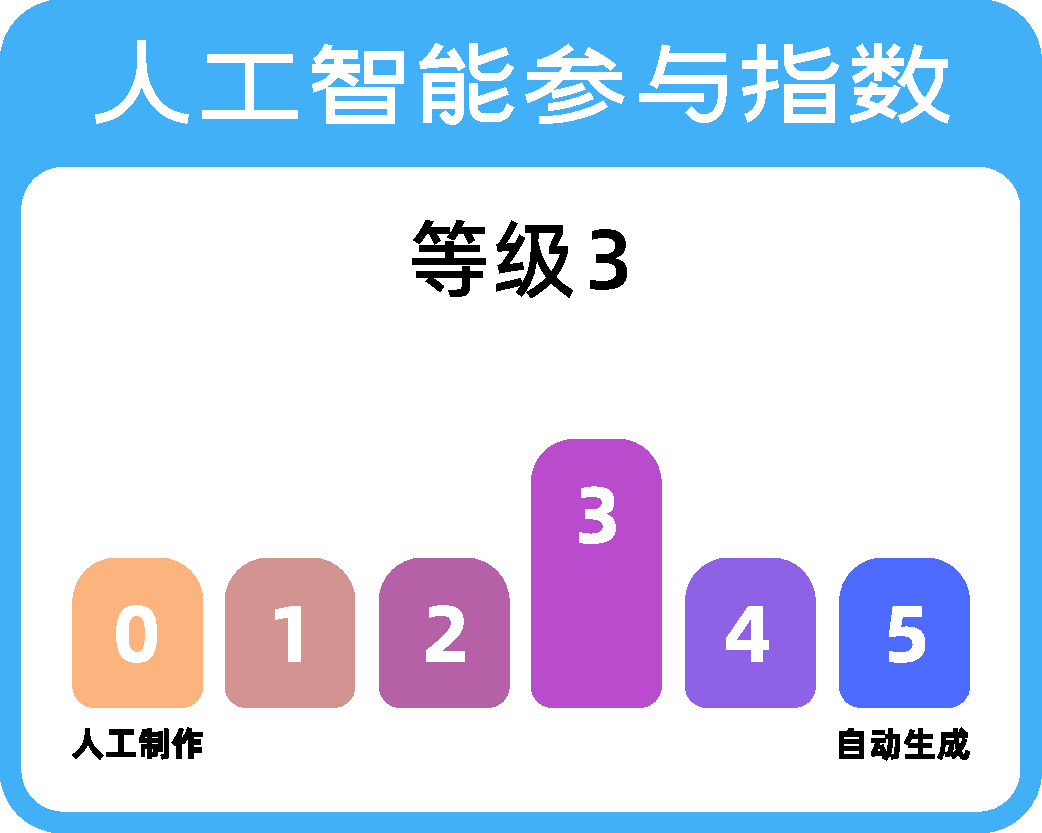
\includegraphics[width=0.4\textwidth]{img/iiia.pdf}
    \end{center}
\end{center}

本笔记借助了GitHub Copilot生成。这玩意太好用了,甚至能猜想到例句(不过发音符号有时会标错),我审核了AI生成的所有内容,但由于毕竟是新接触一套书写系统,难免有拼写疏漏。

\begin{attention}
    这样的格式代表老师在课上强调的知识点。
\end{attention}

\begin{note}
    这样的格式代表我自己的感悟。
\end{note}

\tableofcontents

\chapter{引言和字母表部分}

本章对应课程P1~P7。

\section{字母表(\arm{اَلْأَبْجَدِيَّةُ الْعَرَبِيَّةُ})及特殊字母写法}

\begin{note}
    字母表请务必跟着视频课学习。笔记只能呈现字母的部分形态。

    此外,在学习阿语字母表时,我愈发意识到,对于老师来说,阿语的一些字形可能已经很熟悉,因此讲解时会快速带过,或干脆略过。但我们来说,面对这样一款陌生的语言,我们需要尝试用最快的速度掌握分辨字形的合适粒度。也就是说,我们需要知道对于这套文字,哪些地方是装饰、哪些地方是区别字母的关键、哪些地方是字体的差异。

    举个例子,\arm{ل} 与 \arm{ا} 搭配而成的 \arm{لا} 有一个独特的词尾型 \arm{ـلا}。在字形呈现上, \arm{لا} 和 \arm{ـلا} 可能很相似,也可能相差很大。这是视频课中没有明确提到的,需要我们自己去观察发现。
\end{note}

\begin{Arabic}
    \begin{tabular}{c|r|r|r|r}
        \crm{独立型} & \crm{读音} & \crm{词头、中、尾连写} & \crm{誊抄} & \crm{特殊形态} \\
        \hline
        أ & أَلِفٌ & أـأـأ & \ait{أـأـأ} & إِ آ \\
        ب & بَاءٌ & بـبـب & \ait{ببب}\\
        ت & تَاءٌ & تـتـت & \ait{تتت} & ة/ـة ةََ \\
        ث & ثَاءٌ & ثـثـث & \ait{ثثث}\\
        ج & جِيمٌ & جـجـج & \ait{ججج}\\
        ح & حَاءٌ & حـحـح & \ait{ححح}\\
        خ & خَاءٌ (厚) & خـخـخ & \ait{خخخ}\\
        د & دَالٌ & دـدـد & \ait{دـدـد}\\
        ذ & ذَالٌ (咬) & ذـذـذ & \ait{ذـذـذ}\\
        ر & رَاءٌ (厚) & رـرـر & \ait{رـرـر}\\
        ز & زَاىٌ & زـزـز & \ait{زـزـز}\\
        س & سِينٌ & سـسـس & \ait{سسس}\\
        ش & شِينٌ & شـشـش & \ait{ششش}\\
        ص & صَادٌ (厚) & صـصـص & \ait{صصص}\\
        ض & ضَادٌ (厚) & ضـضـض & \ait{ضضض}\\
        ط & طَاءٌ (厚) & طـطـط & \ait{تتت}\\
        ظ & ظَاءٌ (厚/咬) & ظـظـظ & \ait{ظـظـظ}\\
        ع & عَينٌ & عـعـع & \ait{ععع}\\
        غ & غَينٌ & غـغـغ & \ait{غغغ}\\
        ف & فَاءٌ & فـفـف & \ait{ففف}\\
        ق & قَافٌ (厚) & قـقـق & \ait{ققق}\\
        ك & كَافٌ & كـكـك & \ait{ككك}\\
        ل & لَامٌ & لـلـل & \ait{للل} & لا/ـلا لاَ لاََ \\
        م & مِيمٌ & مـمـم & \ait{ممم}\\
        ن & نُونٌ & نـنـن & \ait{ننن}\\
        ه & هَاءٌ & هـهـه & \ait{ههه}\\
        و & وَاوٌ & وـوـو & \ait{وـوـو}\\
        ى & يَاءٌ & يـيـى & \ait{ييى}\\
    \end{tabular}
\end{Arabic}

\begin{itemize}
    \item 标``厚''表示其后加 \arm{ـَ} 或 \arm{ـَا} 时发音要更浑厚(靠后,类似\textipa{[A]})。
    \item 标``咬''表示咬舌发音。
    \item \arm{ة} 常位于词尾,一般为阴性名词标志,其前字母永远标 \arm{ـَ} 或 \arm{ـَا} 。\arm{ة} 搭配 \arm{ــََا} 时不写 \arm{ا}。
\end{itemize}

\begin{note}
    在学习满语时我发现,如果过多按照独立型去背诵字母形态,在识读单词的时候会遇到更大的障碍,因为单词中的单词大多数处于词中型。既然如此,为什么不按照词中型将字母整理出来呢?于是,便有了这个列表。

    我根据自己的理解,依照课上的手写体,给每个形状取了名字。此外,请注意阅读顺序(从两边到中间)。
    \begin{itemize}
        \item \ac{ـهـ و ـمـ}{(不规则)h, w, m}
        \item \ac{ـئـ / ـنـ ـتـ ـثـ / ـبـ ـيـ}{(短牙型)' / n, t, th / b, y}
        \item \ac{ـلـ ـكـ}{(长牙型)l, k}
        \item \ac{ـــحـ / ـــخـ / ـــجـ}{(闪电型)ḥ / kh / \textipa{\textdyoghlig}}
        \item \ac{د ذ / ر ز}{(小钩型)d, dh / r, z}
        \item \ac{ـسـ ـشـ}{(横线型)s, sh}
        \item \ac{ـفـ ـقـ / ـطـ ـظـ / ـصـ ـضـ}{(上圈型)f, q / ṭ, ẓ / ṣ, ḍ}
        \item \ac{ـعـ ـغـ}{(三角型)`, gh}
    \end{itemize}

    可以看到,转写中为拉丁字母加点,对应到阿文很可能会完全变成另一个字母。于是,我又整理了如下表格,来表示部分字母的发音关系。该表中,关于中心轴对称的辅音互为清浊关系。越远离中心轴,表示发音越难(加喉音、加顶音等)。对应转写并列展示。

    \begin{center}
    \begin{multicols}{2}
    \begin{tabular}{cc||cc}
        \hline
        \arm{ض} & \arm{د} & \arm{ت} & \arm{ط} \\
        && \arm{ك} & \arm{ق} \\
        & \arm{غ} & \arm{خ} \\
        \arm{ع} && \arm{ه} & \arm{ح}\\
        & \arm{ج} & \arm{ش} \\
        & \arm{ز} & \arm{س} & \arm{ص} \\
        \arm{ظ} & \arm{ذ} & \arm{ث} \\
        \hline
    \end{tabular}

    \begin{tabular}{cc||cc}
    
        \hline
        ḍ & d & t & ṭ \\
        && k & q \\
        & gh & kh \\
        ` && h & ḥ \\
        & \textipa{\textdyoghlig} & sh \\
        & z & s & ṣ \\
        ẓ & dh & th \\
        \hline

    \end{tabular}
    \end{multicols}
    \end{center}
\end{note}

\section{单词和课文}

\subsection{引入和字母部分}

\begin{itemize}
    \item \ac{اَلْعَرَبِيَّةُ}{阿拉伯语}
    \item \ac{اَلْبُلْدَانُ الْعَرَبِيَّةُ}{阿拉伯国家}
    \item \ac{صَحْرَاءُ}{沙漠}
    \item \ac{اَصَّحْرَاءُ الْكُبْرَى}{撒哈拉沙漠(沙漠--最大的)}
    \item \ac{جَمَلٌ}{骆驼}
    \item \ac{نِفْطٌ}{石油}
    \item \ac{بِتْرُولٌ}{石油(音译自petrol)}
    \item \ac{قَهْوَةٌ}{咖啡}
    \item \ac{أَلْفُ لَيْلَةِِ وَلَيْلَةٌ}{《一千零一夜》(一千--夜(属)--和一夜)}
    \item \ac{جُبْرَانُ}{纪伯伦}
    \item \ac{اَللُّغَاتُ السَّامِيَّةُ}{闪米特语族(Semitic Languages)}

\end{itemize}

\section{语法}

阿拉伯语属于闪含语系闪语族(闪米特语族),诞生于阿拉伯半岛,最早的文献可以追溯到公元6世纪阿拉伯半岛北部的石刻。

阿拉伯语辅音相对复杂,一般三个辅音字母构成基本含义。例如:

\begin{itemize}
    \item \ac{فَهِمَ}{理解}
    \item \ac{أَفِهَمَ}{使……理解}
    \item \ac{تَفَاهَمَ}{相互理解}
    \item \ac{اِسْتَفْهَمَ}{询问(要求理解)}
    \item \ac{مَفْهُومٌ}{概念(被理解的事物)}
\end{itemize}

阿拉伯语有名词、动词、虚词,没有系动词:

\begin{itemize}
    \item \ac{هَذَا كِتَابٌ.}{这--一本书。(\arm{هَذَا}注音为\arm{هَاذَا})}
\end{itemize}

阿语动词常在句首:遇到--张三(主格)--李四(宾格)

\setcounter{chapter}{7}
\chapter{hello, world}

\section{\lecon{8.2} 单词和课文}

\begin{multicols}{2}
    \begin{itemize}
        \item \ac{أَهْلٌ}{家人}
        \item \ac{وَـ}{和--}
        \item \ac{سَهْلٌ}{平原}
        \item \ac{مَنْ}{谁}
        \item \ac{أَنْتَ / أَنْتِ}{你}
        \item \ac{أَنَا}{我}
        \item \ac{هُوَ / هِىَ}{他}
        \item[]
    \end{itemize}
\end{multicols}


\begin{Arabic}
    - أَهْلاً وَسَهْلاً!

    - أَهْلاً وَسَهْلاً!

    - مَنْ أَنْتَ؟

    - أَنَا مَنْصُورٌ، وَمَنْ أَنْتِ؟

    - أَنَا يُمْنَى.

    - مَنْ هُوَ؟

    - هُوَ أَحْمَدُ.

    - وَمَنْ هِىَ؟

    - هِىَ يُمْنَى.
\end{Arabic}

\section{语法}

\subsection{\lecon{8.3} \arm{ن} 的显读( \arm{أَلْإِظْهَارُ})}

\arm{ن} 在以下字母前面发音明显:\arm{أ ه ح خ ع غ}

\begin{multicols}{2}
    \begin{itemize}
        \item \ac{أَنْحَاءٌ}{}
        \item \ac{أَنْخَابٌ}{}
        \item \ac{صَنْعَاءٌ}{萨那(也门首都)}
        \item \ac{أَنْغَاءٌ}{}
    \end{itemize}
\end{multicols}

\subsection{\lecon{8.4} 词法}

阿语有三种词性。

\begin{itemize}
    \item 动词
    \begin{itemize}
        \item 人称:1/2/3
        \item 性:阴/阳
        \item 数:单/双/复
        \item 格:主/宾/切
        \item 时式:过去/现在/命令
    \end{itemize}
    \item 名词
    \begin{itemize}
        \item 性:阴/阳
        \item 数:单/双/复
        \item 格:主/宾/属
        \item 式:泛指/确指
    \end{itemize}
    \item 虚词
    \begin{itemize}
        \item 介词(需要加名词属格)
        \item 联词
        \item 疑问虚词、应答虚词
        \item …………
    \end{itemize}
\end{itemize}

阿语句子分为以动词开头的动词句和以名词开头的名词句。
\chapter{君の名は?}

\section{\lecon{9.2} 单词和课文}

\begin{itemize}
    \item \ac{مَا}{谁}
    \item \ac{اِسْمٌ}{名字}
    \item \ac{اِسْمُكَ / اِسْمُكِ}{你的名字}
    \item \ac{اِسْمِى}{我的名字}
    \item \ac{اِسْمُهُ / اِسْمُهَا}{他的名字}
    \item \ac{بِ}{prep. 借助}
    \item \ac{أَهْلًا بِكَ!}{你好}
    \item \ac{حَسَنًا}{好的}
    \item \ac{إِلَى}{prep. 向、到}
    \item \ac{اَلْ}{冠词(无\arm{ء
    })}
    \item \ac{لِقَاءٌ}{n. 见面}
    \item \ac{إِلَى اللِّقَاءِ}{再见}
\end{itemize}

\begin{Arabic}
    - أَهْلاً وَسَهْلاً! 

    - أَهْلاً وَسَهْلاً!

    - مَا اسْمُكَ؟

    - اِسْمِى أَهْمَدُ. وَمَا اسْمُكَ؟

    - اِسْمِى مَنْصُورٌ.

    - أَهْلاً وَسَهْلاً!

    - أَهْلاً بِكَ!

    - أَنَا مَنْصُورٌ. وَمَا اسْمُكِ؟

    - اِسْمِى يُمْنَى.

    - حَسَنًا.إِلَى للِّقَاءِ!

    - إِلَى للِّقَاءِ! 
\end{Arabic}

\begin{attention}
    \arm{مَا اسْمُكَ؟} 读音为\arm{مَسْمُكَ}。

    \arm{إِلَى} (介词)后面 \arm{لِقَاءٌ} 变为属格 \arm{لِقَاءِ} 。
\end{attention}

\section{语法}

\subsection{音节和重音}

短音节和长音节按直觉来。

\begin{itemize}
    \item 单音节词一律重读。
    \item 双音节词重读第一个音节。
    \item 多音节词:
    \begin{itemize}
        \item 词尾长音节不重读。
        \item 有叠音的重读叠音前。
        \item 两个以上长音节者,重读最后一个长音节。
        \item 重读倒数二三音节中的长音节,若有。
        \item 倒数第二个音节是短音节者,重读倒数第三个音节。
    \end{itemize}
\end{itemize}

\begin{note}
    似乎没有两个长音组成的双音节词?
\end{note}

\begin{note}
    \arm{ـً} 和 \arm{ـَنْ} 的发音没有区别,但课中没有提到二者的区别,我猜测的区别有:
    \begin{itemize}
        \item 正词法规定;
        \item \arm{ـَنْ} 比 \arm{ـً} 多一个辅音 \arm{ن} ,而闪语族语言的辅音可能有特殊含义。
    \end{itemize}
\end{note}

\subsection{名词的性}

名词分阴阳性,没有中性。大多数阴性名词有以下规律:

\begin{itemize}
    \item 绝大部分国名、城市名、部落名。
    \begin{itemize}
        \item \ac{دِمَشْقُ}{大马士革}
        \item \ac{بَكِينُ}{北京}
        \item \ac{سُورِيَا}{叙利亚}
        \item \ac{اَلصِّنُ}{中国}
    \end{itemize}
    \item 大部分成双的肢体和器官。
    \begin{itemize}
        \item \ac{قَدَمٌ}{脚}
        \item \ac{عَيْنٌص}{眼睛}
        \item \ac{كَفٌّ}{手掌}
        \item \ac{يَدٌ}{手}
    \end{itemize}
    \item 指物名词的复数当作阴性单数看待。
\end{itemize}

仅有有限的阴性名词没有规律:

\begin{itemize}
    \item \ac{نَارٌ}{火}
    \item \ac{شَمُسٌ}{日}
    \item \ac{أَرْضٌ}{地}
    \item \ac{سِنٌّ}{牙}
    \item \ac{دَارٌ}{房}
    \item \ac{حَرەبٌ}{战争}
    \item \ac{رِيحٌ}{风}
    \item \ac{رُوحٌ}{灵魂、精神}
    \item …………
\end{itemize}

\subsubsection{阴性标志}

绝大多数具有阴性标志的名词是阴性名词。

\begin{note}
    对于大多数情况:
    
    \begin{center}
        带有阴性标志 \tto 阴性名词
    \end{center}

    且课上没有说反向是否可以。
\end{note}

阴性标志有如下几个。注意:全都有例外。

\paragraph{\arm{ة/ـة}} 

\begin{itemize}
    \item \ac{سَعَادَةٌ}{幸福}
    \item \ac{حَيَاةٌ}{生活}
    \item \ac{شرِكَةٌ}{公司}
\end{itemize}

可以在阳性名词后面加上 \arm{ة/ـة} 使其变成阴性。

\begin{itemize}
    \item \ac{فَتًى \tto فَتَاةٌ}{小伙 \tto 姑娘}
    \item \ac{جَمِيلٌ \tto جَمِيلَةٌ}{美丽的}
    \item \ac{لَيْلٌ \tto لَيْلَةٌ}{夜晚 \tto 一个夜晚}
    \item \ac{خُبْزٌ \tto خُبْزَةٌ}{面包 \tto 一块面包}
\end{itemize}

\paragraph{\arm{ـَى}}

\begin{itemize}
    \item \ac{بُشْرَى}{喜讯}
    \item \ac{ذِكْرَى}{纪念}
    \item \ac{كُبْرَى}{最大的(阴性)/la plus grande}
    \item \ac{يُمْنَى}{(人名)}
\end{itemize}

\paragraph{\arm{ـَاءُ}}

\begin{itemize}
    \item \ac{صَحْرَاءُ}{沙漠}
    \item \ac{سَوْدَاءُ}{黑色的(阴性)/noire}
\end{itemize}

\subsubsection{共性名词}

阴阳性通用的名词叫作共性名词。

\begin{itemize}
    \item \ac{صَبُورٌ}{忍耐的}
    \item \ac{قَتِيلٌ}{被杀的}
    \item \ac{سَمَاءٌ}{天空}
    \item \ac{سُوقٌ}{市场}
\end{itemize}

\subsection{名词的格}

属格作为介词受词。属格作为偏正组合偏次。

\paragraph{定尾名词} 无论什么格都固定尾符的名词。

\begin{itemize}
    \item \ac{مَنْ}{(疑问代词)谁}
    \item \ac{مَا}{(疑问代词)什么}
    \item \ac{هَذَا}{(指示代词)这个}
    \item \ac{يُمْنَى}{(人名)}
\end{itemize}

\begin{note}
    \arm{هَذَا} 注音为 \arm{هَاذَا} 。考虑到前面也对于同一个词出现过这个情况,应该是特殊读音。

    【后补】是的,就是特殊读音。
\end{note}

\paragraph{变尾名词} 通常尾符随格变化的名词。

\begin{center}
    \begin{tabular}{c|ccc}
        & 主 & 宾 & 属 \\
        \hline
        确指 & \arm{ـُ} & \arm{ـَ} & \arm{ـِ}\\
        泛指 & \arm{ـٌ} & \arm{ـًا} & \arm{ـٍ}
    \end{tabular}
\end{center}

以 \arm{بَيْتٌ} (房子)为例。

\begin{center}
    \begin{tabular}{c|ccc}
        & 主 & 宾 & 属 \\
        \hline
        确指 & \arm{اَلْبَيْتُ} & \arm{اَلْبَيْتَ} & \arm{اَلْبَيْتِ}\\
        泛指 & \arm{بَيْتٌ} & \arm{بَيْتًا} & \arm{بَيْتٍ}
    \end{tabular}
\end{center}

对于一些人名地名,确指也标双音符。

\begin{center}
    \begin{tabular}{c|ccc}
        & 主 & 宾 & 属 \\
        \hline
        确指 & \arm{مَنْصُورٌ} & \arm{مَنْصُورًا} & \arm{مَنْصُورٍ}\\
    \end{tabular}
\end{center}

\paragraph{半变尾名词} 尾符随格而有部分变化的名词,如一些人名和地名。特点是词尾不标双音符。

\begin{center}
    \begin{tabular}{c|ccc}
        & 主 & 宾 & 属 \\
        \hline
        大马士革 & \arm{دِمَشْقُ} & \arm{دِمَشْقَ} & \arm{دِمَشْقَ}(不是 \arm{..ـقِ})\\
        艾哈迈德 & \arm{أَحْمَدُ} & \arm{أَحْمَدَ} & \arm{أَحْمَدَ}(不是 \arm{..ـدِ})
    \end{tabular}
\end{center}

但是,半变尾名词加冠词 \arm{اَلْ} 或后面被属格名词修饰(即作偏正组合正次),则属格为 \arm{ـِ}。
\chapter{\textmongolian{ᠪᡳ ᠣᠴᡳ ᡨᠠᠴᡳᠰᡳ ᡳᠨᡠ}}

\section{\lecon{10.1} 单词和课文}

\begin{multicols}{2}
    \begin{itemize}
        \item \ac{هَلْ}{……吗?}
        \item \ac{طَالِبٌ / طَلِبَةٌ}{学生}
        \item \ac{طَبِيبٌ / طَبِيبَةٌ}{医生}
        \item \ac{صَدِيقٌ / صَدِيقَةٌ}{朋友}
        \item \ac{صَدِيقِى / صَدِيقَتِى}{我的朋友}
        \item \ac{زَمِيلٌ / زَمِيلَةٌ}{同学/同事}
        \item \ac{زَمِيلِى / زَمِيلَتِى}{我的同学/同事}
        \item \ac{يَا}{喂(后接人名末尾 \arm{ـٌ} 变 \arm{ـُ})}
        \item \ac{نَعَمْ}{是}
        \item \ac{لَا}{否}
        \item \ac{مُدَرِّسٌ / مُدِرِّسَةٌ}{老师}
        \item \ac{مُهَنْدِسٌ / مُهَنْدِسَةٌ}{工程师}
        \item \ac{مُمَرِّضٌ / مُمَرِّضَةٌ}{护士}
        \item []
    \end{itemize}
\end{multicols}


\begin{Arabic}
    - أَهْلاً وَسَهْلاً!

    - أَهْلاً بِكِ!

    - هَلْ أنْتَ طَالِبٌ؟

    - نَعَمْ. أَنَا طَالِبٌ. هَلْ أَنْتِ طَالِبَةٌ أَيْضًا؟

    - لَا، أَنَا طَبِيبَةٌ.

    - يَا يُمْنَى، هُوَ صَدِيقِى، اِسْمُهُ أَحْمَدُ.

    - أَهْلاً بِكَ، يَا أَحْمَدُ

    - أَهْلاً بِكِ!

    - هَلْ أَنْتَ طَالِبٌ أَيْضًا؟

    - نَعَمْ. أَنَا طَالِبٌ أَيْضًا. أَنَا زَمِيلُهُ.

    - نَعَمْ، هُوَ زَمِيلِي.
\end{Arabic}

\begin{note}
    同样,课上同时出现了 \arm{زَمِيلِي} 和 \arm{زَمِيلِى} ,仍然不清楚 \arm{ـي} 下面的两点是否可以省略。
\end{note}

\begin{attention}
    \arm{أَيْضا} 也,\arm{زَمِيلُهُ} 他的同学。
\end{attention}



\paragraph{\lecon{10.2} ……的……}

\begin{note}
    这是属格接尾人称代词的先导。
\end{note}

以 \arm{زَمِيلٌ / زَمِيلَةٌ} 为例。

\begin{center}
    \begin{Arabic}
    \begin{tabular}{r|c|rr}
         & \crm{变位方式} & 阳 & 阴 \\
        \hline
        \crm{原型} & & زَمِيلٌ & زَمِيلَةٌ \\
        أَنَا & ـٌ $\leftarrow$  ـِى  & زَمِيلِى & زَمِيلَتِى \\
        أَنْتَ &   &  &  \\
        أَنْتِ &  &  &  \\
        هُوَ & ـٌ $\leftarrow$ ـُهُ & زَمِيلُهُ & زَمِيلَتُهُ \\
        هِيَ & ـٌ $\leftarrow$ ـُهَا & زَمِيلُهَا & زَمِيلَتُهَا \\
    \end{tabular}
\end{Arabic}
\end{center}

\section{语法}

\subsection{\lecon{10.3} 名词双数}

主格:\arm{ـٌ} \tto \arm{ـَانِ}

宾格、属格:\arm{ـٌ} \tto \arm{ـَيْنِ}

\begin{center}
    \begin{tabular}{cc|cc}
        两个…… & & 主格 & 宾、属格 \\
        \hline
        房子 & \arm{بَيْتٌ} & \arm{بَيْتَانِ} & \arm{بَيْتَِيْنِ} \\
        男人 & \arm{رَجُلٌ} & \arm{رَجُلَانِ} & \arm{رَجُلَيْنِ} \\
        小伙子 & \arm{فَتًى} & \arm{فَتَيَانِ} & \arm{فَتَيَيْنِ} \\
        姑娘 & \arm{فَتَاةٌ} & \arm{فَتَاتَانِ} & \arm{فَتَاتَيْنِ} \\
        公司 & \arm{شَرِكَةٌ} & \arm{شَركَتَانِ} & \arm{شَركَتَيْنِ} \\
    \end{tabular}
\end{center}

所谓``弄假成真'',即诸如 \arm{فَتًى} 末尾 \arm{ى} 形的 \arm{أ} 直接作为 \arm{ى} 而处理成 \arm{ـيـ}。

\subsection{\lecon{10.4} 主格独立人称代词}

\begin{center}
    \begin{Arabic}
    \begin{tabular}{c|c|c|c}
        \crm{人称} & \crm{单数} & \crm{双数} & \crm{复数} \\
        \hline
        \crm{一} & أَنَا = أَنَا & \crm{无} & نَحْنُ = نَحْنُ \\
        \crm{二} & أَنْتَ / أَنْتِ & أَنْتُمَا = أَنْتُمَا & أَنْتُمْ / أَنْتُنَّ \\
        \crm{三} & هُوَ / هِيَ & هُمَا = هُمَا & هُمْ / هُنَّ 
    \end{tabular}
\end{Arabic}
\end{center}

\subsection{\lecon{10.5} 属格接尾人称代词}

\begin{multicols}{2}
    \begin{itemize}
        \item \ac{مِنْ}{prep. 来自}
        \item \ac{عَلَى}{在……上}
    \end{itemize}
\end{multicols}

不独立使用,后缀与名词词尾。后缀变位:

\begin{center}
    \begin{Arabic}
        \begin{tabular}{c|c|c|c}
            \crm{人称} & \crm{单数} & \crm{双数} & \crm{复数} \\
            \hline
            \crm{一} & أَنَا : ـِى  & \crm{无} & نَحْنُ : ـنَا \\
            \hline
            \multirow{2}{*}{\crm{二}} & أَنْتَ : ـكَ & \multirow{2}{*}{أَنْتُمَا : ـكُمَا} & أَنْتُمْ : ـكُمْ \\
                & أَنْتِ : ـكِ & & أَنْتُنَّ : ـكُنَّ \\

            \hline
            \multirow{2}{*}{\crm{三}} & هُوَ : ـهُ & \multirow{2}{*}{هُمَا : ـهُمَا} & هُمْ : ـهُمْ \\
                & هِىَ : ـهَا & & هُنَّ : ـهُنَّ \\
        \end{tabular}
    \end{Arabic}
\end{center}

\begin{note}
    不知道为什么,课上喜欢从更为复杂的第三人称开始,讲到较为简单的第一人称。但笔记仍然遵循一、二、三人称的顺序了。

    具体来说,第三人称比较好记,双、复数完全就是直接把独立主格人称代词放到后面,单数却是一个短音一个长音。

    如果说第三人称的主题是 \arm{ه},那第二人称的主题就是 \arm{ك}。用满语来辅助记忆:双、复数直接就是``去掉第三人称的圈''。

    单数和第一人称硬记。

    属格不改变原词的性。如 \arm{بَيْتٌ}(阳性)接阴性后缀后(如 \arm{بَيْتُكِ})仍为阳性。
\end{note}

\paragraph{鼻音符不能接属格接尾人称代词} 去掉 \arm{ـً، ـٍ، ـٌ} 的双写,或直接被第一人称单数的 \arm{ـِى} 替代。

\paragraph{冠词和属格接尾人称代词不能同时存在} 很好理解,ma maison可以但la ma maison不可以。

\paragraph{第三人称音变} 以下结尾的名词变第三人称属格时 \arm{ـهُ/ـهُـ} 变 \arm{ـهِ/ـهِـ}:

\begin{Arabic}
    \begin{itemize}
        \item ـِ
        \item ـِى
        \item ـَىْ
    \end{itemize}
\end{Arabic}

以 \arm{بَيْتٌ} 的词组 \arm{فِي بَيْتِ}(在房子里)为例:

\begin{center}
    \begin{Arabic}
        \begin{tabular}{c|c|c|c}
            \crm{在房子里} & \crm{第三人称单数} & \crm{第三人称双数} & \crm{第三人称复数} \\
            \hline
            \multirow{2}{*}{فِي بَيْتِ} & هُوَ : فِي بَيْتِهِ & \multirow{2}{*}{هُمَا : فِي بَيْتِهِمَا} & هُمْ : فِي بَيْتِهِمْ \\
                & هِىَ : فِي بَيْتِهَا & & هُنَّ : فِي بَيْتِهِنَّ \\
        \end{tabular}
    \end{Arabic}
\end{center}

\begin{note}
    其实就是 ``真[i]'' (而不含 \arm{ى} 形 \arm{ا} 这样的``假[i]'')结尾,真的很像元音和谐律。
\end{note}

\paragraph{附加的 \arm{ن} 接属格接尾人称代词要去掉} 例如名词双数、阳性完整式复数的情况。

\begin{note}
    记得连着 \arm{ن} 的元音一起去掉,即去掉整个音节。
\end{note}

\begin{note}
    \begin{center}
        \begin{center}

\begin{tikzpicture}[
    scale=3,              % 图形缩放比例
    every node/.style={}, % 所有节点字体大小
    vertex/.style={circle, fill=black, inner sep=1.5pt}, % 顶点样式
    edge label/.style={midway, fill=white, inner sep=1pt}, % 边注释样式
]

% 定义正方体顶点坐标(三维坐标:x, y, z)
\coordinate (A) at (0,0,0);
\coordinate (B) at (-1,0,0);
\coordinate (C) at (-1,-1,0);
\coordinate (D) at (0,-1,0);
\coordinate (E) at (0,0,-1);
\coordinate (F) at (-1,0,-1);
\coordinate (G) at (-1,-1,-1);
\coordinate (H) at (0,-1,-1);

\draw (A) node[vertex, label=below right:\arm{بَيْتٌ}{\footnotesize 房}] {};
\draw (B) node[vertex, label=left:{\footnotesize 俩房} \arm{بَيْتَانِ}] {};
\draw (D) node[vertex, label=right:\arm{بَيْتُهُ}{\footnotesize 他的房}] {};
\draw (C) node[vertex, label=left:{\footnotesize 他的俩房} \arm{بَيْتَاهُ}] {};

\draw (E) node[vertex, label=right:\arm{فِى بَيْتِِ}{\footnotesize 房里}] {};
\draw (F) node[vertex, label=left:{\footnotesize 俩房里} \arm{فِى بَيْتَيْنِ}] {};
\draw (H) node[vertex, label=right:{\footnotesize 他房里}\arm{فِى بَيْتِهِ}] {};
\draw (G) node[vertex, label=below:{\footnotesize 他的俩房里} \arm{فِى بَيْتَيْهِ}] {};

\draw[thick] (C) -- (D);
\draw[thick, dashed] (E) -- (F);
\draw[thick, dashed] (G) -- (H);
\draw[thick, dashed] (H) -- (E);

\draw[thick, -{Stealth[length=3mm]}] (B) -- (C) node[edge label, sloped, right, rotate=180]{\footnotesize (去 \arm{ن})};
\draw[thick, -{Stealth[length=3mm]}, dashed] (F) -- (G)node[edge label, sloped, left, rotate=180]{\footnotesize (去 \arm{ن})};

\draw[thick, -{Stealth[length=3mm]}] (A) -- (B) node[edge label]{双};
\draw[thick, -{Stealth[length=3mm]}] (A) -- (D) node[edge label, sloped, rotate=180]{属他};
\draw[thick, -{Stealth[length=3mm]}, dashed] (A) -- (E) node[edge label, sloped]{宾};

\end{tikzpicture}

\end{center}
    \end{center}
\end{note}

\begin{note}
    \arm{بَيْتٌ} \tto 宾格泛指 \arm{فِى بَيْتٍ},加属格接尾人称代词``在他的房子里''步骤如下:
    \begin{enumerate}
        \item 结尾不能鼻音符:\arm{فِى بَيْتٍ} \tto \arm{فِى بَيْتِ};
        \item \arm{ـِ} 结尾,\arm{ـهُ} 变 \arm{ـهِ}:\arm{فِى بَيْتِهُ} \tto \arm{فِى بَيْتِهِ}。
    \end{enumerate}
\end{note}

(还没学到)再如,完整式阳性复数加接尾人称代词:

\begin{itemize}
    \item 主格: \arm{ـُونَ} \tto \arm{ـُوـ..}
    \item 宾属格: \arm{ـِينَ}  \tto \arm{ـِيـ..}
\end{itemize}

\begin{Arabic}
    \begin{center}
        \begin{tabular}{c|cc}
            \crm{老师} & \crm{老师们} & \crm{她的老师们} \\
            \hline
            مُدَرِّسٌ & مُدَرِّسُونَ & مُدَرِّسُوهَا \\
             & مِنْ مُدَرِّسِينَ & مِنْ مُدَرِّسِيهَا
        \end{tabular}
    \end{center}
\end{Arabic}



\paragraph{第一人称读法变化} ``我的''接在下列词尾后时,不吞掉原词尾,直接加 \arm{ـىَ}

\begin{Arabic}
    \begin{itemize}
        \item ـَا
        \item ـُو
        \item ـَى
    \end{itemize}
\end{Arabic}

\begin{itemize}
    \item \ac{بَيْتَانِ \tto بَيْتَاىَ \tto عَلَى بَيْتَيْىَ}{俩房 \tto 我的俩房 \tto 我的俩房上}
    \begin{itemize}
        \item 第一个变化是先去 \arm{ن} 再由于 \arm{ـتَا} 而接 \arm{ـىَ}
        \item 第二个变化是先去 \arm{ن} 再由于 \arm{ـتَىْ} 而接 \arm{ـىَ}
    \end{itemize}
    \item \ac{مُدَرِّسُونَ \tto مُدَرِّسُوىَ \tto مِنْ مُدَرِّسِيىَ}{老师们 \tto 我老师们  \tto 来自我的老师们 \\}
\end{itemize}


在以下介词后时,也有读音变化:

\begin{itemize}
    \item \ac{بِ \tto بِيَ}{凭借、在 \tto 凭借我、在我这}
    \item \ac{فِي \tto فِيَّ}{在……里 \tto 在我的里面}
    \item \ac{مِنْ \tto مِنِّي}{从 \tto 从我这}
    \item \ac{عَنْ \tto عَنِّي}{关于、通过 \tto 关于我、通过我}
\end{itemize}

\begin{note}
    注意,指的是在两个介词后面直接变位(如``凭借我'')。此外,\arm{فِي} 和变音后缀的 \arm{ـنِي} 的长音下面是加两点的,不知道为什么。

    此外,我是真没想到介词也能这么变。
\end{note}
\chapter{你是哪国人}

\section{\lecon{11.1}询问国籍}

\begin{itemize}
    \item \ac{جِنْسِيَّةٌ}{国籍}
\end{itemize}

末尾的 \arm{ـة}标记了阴性名词。

\begin{Arabic}
    \begin{itemize}
        \item مَا جِنْسِيَّتُكَ/جِنْسِيَّتُكِ؟
        \item مَا جِنْسِيَّتُهُ/جِنْسِيَّتُهَا؟
    \end{itemize}
\end{Arabic}

一些国家自带冠词。

\begin{Arabic}
    \begin{center}
        \begin{tabular}{lr|rr}
             & & هُوَ ... & هِىَ ...\\
            \hline
            \crm{中国} & اَلصِّينُ & صِينِيٌّ & صِينِيَّةٌ \\
            \crm{沙特} & اَلسُّعُودِيَّةُ & سُعُودِيٌّ & سُعُودِيَّةٌ \\
            \crm{阿联酋} & اَلْإِمَارَاتُ & إِمَارَاتِيٌّ & إِمَارَاتِيَّةٌ \\
            \crm{也门(阳性)} & اَلْيَمَنُ & يَمَنيٌّ & يَمَنيَّةٌ \\
            \crm{埃及} & مِصْرُ & مِصْرِيٌّ & مِصْرِيَّةٌ \\
            \crm{叙利亚} & سُورِيَا & سُورِيٌّ & سُورِيَّةٌ\\
            \crm{伊拉克(阳性)} & اَلْعِرَاقُ & عِرَاقِيٌّ & عِرَاقِيَّةٌ \\
            \crm{} & بِرِيطَانِيَا & بِرِيطَانِيٌّ & بِرِيطَانِيَّةٌ \\
            \crm{} & فَرَنْسَا & فَرَنْسِيٌّ & فَرَنْسِيَّةٌ \\
            \crm{} & أَلْمَانِيَا & أَلْمَانِيٌّ & أَلْمَانِيَّةٌ \\
            \crm{} & أَسْبَانِيَا & أَسْبَانِيٌّ & أَسْبَانِيَّةٌ \\
            \crm{} & إِيطَالِيَا & إِيطَالِيٌّ & إِيطَالِيَّةٌ \\
            \crm{} & أَمْرِيكَا & أَمْرِيكِيٌّ & أَمْرِيكِيَّةٌ \\
            \crm{} & رُوسِيَا & رُوسِيٌّ & رُوسِيَّةٌ \\
            \crm{} & الْيَابَانٌ & يَابَانِيٌّ & يَابَانِيَّةٌ \\
            \crm{} & كُورِيَا & كُورِيٌّ & كُورِيَّةٌ \\
        \end{tabular}
    \end{center}
\end{Arabic}

注意德国开头不是冠词(冠词不带 \arm{ء})。

\begin{note}
    注意一些多了个长音。注意去掉冠词。
\end{note}

\section{\lecon{11.2}名词的完整式复数}

阳性名词通常指人。阴性名词通常指物和用于外来名词。

\begin{Arabic}
    \begin{center}
        \begin{tabular}{c|cc}
             & \crm{主格} & \crm{宾、属格} \\
            \hline
            \crm{阳性} & ـٌ \tto ـُونَ & ـًا/ـٍ \tto ـِينَ\\
            \crm{阴性} & ـ/ـة \tto ـَاتٌ (اَلْـ...ـَاتُ) & ـ/ـة \tto ـَاتٍ(اَلْـ...ـَاتٍ)
        \end{tabular}
    \end{center}
\end{Arabic}

以以下四词为例:

\begin{Arabic}
    \begin{center}
        \begin{tabular}{c|ccc}
            & \crm{单数} & \crm{复数主格} & \crm{复数宾格} \\
            \hline
            \crm{教师} & مُدَرِّسٌ/مُدَرِّسَةٌ & مُدَرِّسُونَ/مُدَرِّسَاتٌ & مُدَرِّسِينَ/مُدَرِّسَاتٍ \\
            \crm{工程师} & مُهَنْدِسٌ/مُهَنْدِسَةٌ & مُهَنْدِسُونَ/مُهَنْدِسَاتٌ & مُهَنْدِسِينَ/مُهَنْدِسَاتٍ \\
            \crm{职员} & مُوَظَّفٌ/مُوَظَّفَةٌ  & مُوَظَّفُونَ/مُوَظَّفَاتٌ & مُوَظَّفِينَ/مُوَظَّفَاتٍ \\
            \crm{努力者} & مُجْتَهِدٌ/مُجْتَهِدَةٌ  & مُجْتَهِدُونَ/مُجْتَهِدَاةتٌ & مُجْتَهِدِينَ/مُجْتَهِدَاةتٍ
        \end{tabular}
    \end{center}
\end{Arabic}

其他阴性名词示例:

\begin{itemize}
    \item \ac{مُسْتَشْفًى \tto مُسْتَشْفَاتٌ}{医院}
    \item \ac{تِلْفُونٌ \tto تِلْفُونَاتٌ}{电话}
    \item \ac{تِلْفِزْيُونٌ \tto تِلْفِزْيُوناتٌ}{电视}
    \item \ac{كُومْبِيُوتَرْ \tto كُومْبِيُوتَراتٌ}{电脑}
\end{itemize}

其中,外来词不必特别拘泥于拼写规则,如外来词中可以有长音--静音的组合。

\section{\lecon{11.3}指示代词}

\begin{multicols}{2}
    
\begin{Arabic}
    \begin{center}
    \begin{tabular}{c|cc}
        \crm{这} & \crm{主格} & \crm{宾、属格} \\
        \hline 
        \crm{单数} & \multicolumn{2}{c}{هَذَا / هَذِهِ }  \\
        \crm{双数} & هَذَانِ / هَاتَانِ & هَذَيْنِ / هَاتَيْنِ \\
        \crm{复数} &  \multicolumn{2}{c}{هَؤُلَاءِ }
    \end{tabular}
    \end{center}
\end{Arabic}

\begin{Arabic}
    \begin{center}
    \begin{tabular}{c|c}
        \crm{那} & \crm{主、宾、属格} \\
        \hline 
        \crm{单数} & \blue{ذَ}لِكَ / تِلْكَ  \\
        \crm{双数} & \multirow{2}{*}{ أُو\blue{لَـ}ـئِكَ} \\
        \crm{复数} 
    \end{tabular}
    \end{center}
\end{Arabic}
\end{multicols}

其中所有 \arm{هَـ}及\blue{蓝色音节}读作长音 \arm{هَا}。

\begin{itemize}
    \item 指示代词+名词=这是……
    \item 指示代词+冠词--名词=这(几)个……
\end{itemize}

以 \arm{مُهَنْدِسٌ/مُهَنْدِسَةٌ}为例:

\begin{Arabic}
    \begin{center}
        \begin{tabular}{c|ccc}
            \crm{\blue{(乃)}} & \crm{这} & \crm{那} \\
            \hline
            \crm{单数} & هَذَا \blue{الْـ}ـمُهَنْدِسٌ. / هَذِهِ \blue{الْـ}ـمُهَنْدِسَةٌ.  & ذَلِكَ \blue{الْـ}ـمُهَنْدِسٌ. / تِلْكَ \blue{الْـ}ـمُهَنْدِسَةٌ. \\
            \crm{双数} & هَذَانِ \blue{الْـ}ـمُهَنْدِسـ(ـَيـ)ـَانِ. & أُولَئِكَ \blue{الْـ}ـمُهَنْدِسـ(ـَيـ)ـَانِ. \\
            \crm{复数} & هَئُلَاءِ \blue{الْـ}ـمُهَنْدِسُونَ/\blue{الْـ}ـمُهَنْدِسَاتٌ. & أُولَئِكَ \blue{الْـ}ـمُهَنْدِسُونَ/\blue{الْـ}ـمُهَنْدِسَاتٌ. \\
        \end{tabular}
    \end{center}
\end{Arabic}

\begin{itemize}
    \item 指示代词+名词--属格接尾代词=这是某人的……
    \item 名词--属格接尾代词+指示代词=某人的这个……
\end{itemize}

以 \arm{بَيْتٌ}和 \arm{صَدِيقٌ}为例:



\begin{Arabic}
    \begin{center}
        \begin{tabular}{c|ccc}
             & \multicolumn{2}{c|}{\crm{\blue{…是他的…}}} & \\
            \hline
            \crm{这个/房子} & \blue{هَذَا} & بَيْتُهُ\blue{.} & \red{هَذَا.} \\
            \crm{这两个/房子} & \blue{هَذَانِ} & بَيْتَاهُ\blue{.} & \red{هَذَانِ.} \\
            \crm{那个/朋友} & \blue{ذَلِكَ} & صَدِيقُهُ\blue{.} & \red{ذَلِكَ.} \\
            \hline
            \multicolumn{2}{c}{} & \multicolumn{2}{|c|}{\crm{\red{他的…/…}}}
        \end{tabular}
    \end{center}
\end{Arabic}
\chapter{卧槽,学霸!}

\section{\lecon{12.2} 单词和课文}

\begin{itemize}
    \item \ac{كَيْفَ}{n. 怎么样}
    \item \ac{حَالٌ}{情况}
    \item \ac{خَيْرٌ}{最好的}
    \item \ac{بِخَيْرٍ}{……很好(\arm{بِـ} 后属格,因此是 \arm{ـٍ})}
    \item \ac{شُكْرًا}{谢谢}
    \item \ac{قَلَمٌ جـ أَقْلَامٌ}{笔}
    \item \ac{مِقْلَمَةٌ جـ مَقَالِمُ}{笔袋}
    \item \ac{كِتَابٌ جـ كُتُبٌ}{书}
    \item \ac{دِرَاسَةٌ}{n. 学习(表抽象意义的词根形式)}
    \item \ac{لِمَنْ ...؟}{……是谁的?}
    \item \ac{... لِي.}{……是我的。}
    \item \ac{يَالَكَ مِنْ ...!}{你真是个……的人啊!}
    \item \ac{مُجْتَهِدٌ فِي ...}{在……上努力的人}
    \item \ac{بَابٌ جـ أَبْوَابٌ}{m. 门}
    \item \ac{نَافِذَةٌ جـ نَوَافِذُ}{f. 窗}
    \item \ac{مَكْتَبٌ جـ مَكَايِبُ}{m. 课桌}
    \item \ac{كُرْسِيٌّ جـ كَرَاسٍ }{(缺尾)m. 椅}
    \item \ac{اِسْمٌ جـ أَسْمَءٌ}{名字}
\end{itemize}

\begin{attention}
    \arm{جـ} 表示后侧是前侧的破碎式复数。

    书等指物名词复数语法上当成阴性单数看待。

    \begin{Arabic}
        \begin{itemize}
            \item هَزِهِ أَبْوَابٌ.
        \end{itemize}
    \end{Arabic}

    复数的 \arm{كَرَاسٍ} 为所谓``缺尾名词'',即其词尾永远是 \arm{ـٍ},并不代表它是属格。
\end{attention}

\begin{note}
    似乎只有破碎式复数而没有``破碎式双数''?
    \begin{itemize}
        \item \ac{هَزَانِ بَابَانِ.}{这是两扇门。}
    \end{itemize}
\end{note}

\begin{Arabic}
    - أَهْلًا وَسَهْلًا!

    - أَهْلًا بِكَ.

    - كَيْفَ حَالُكَ؟

    - أَنَا بِخَيْرٍ، شُكْرًا. وَأَنْتَ؟

    - أَنَا بِخَيْرٍ.

    - مَا هَزَا؟

    - هَزَا قَلَمٌ.

    - وَ مَا هَزِهِ؟

    - هَزِهِ مِقْلَمَةٌ.

    - وَ مَا هَزَا؟

    - هَزَا كِتَابٌ.

    - وَمَا هَزِهِ؟

    - هَزِهِ كُتُبٌ.

    - لِمَنْ هَزِهِ الْكُتُبُ؟

    - هَزِهِ الْكُتُبُ لِي.

    - يَا لَكِ مِنْ مُجْتَهِدَةٍ فِي الدِّرَاسَةِ!
\end{Arabic}

\paragraph{某物是谁的?} \arm{لِـ}--疑问代词(此课只有 \arm{لِمَنْ})+指示代词+ \arm{الـ}--物(注意词尾 \arm{ـٌ} 改成 \arm{ـُ})。

\paragraph{某物是……的} 指示代词+ \arm{الـ}--物+ \arm{لِـ}--属格接尾人称代词。

\begin{Arabic}
    \begin{itemize}
        \item هَزَا الْقَلَمُ / هَزِهِ الْمِقْلَمَةُ ...
        \begin{itemize}[label=\crm{--}]
            \item لِي
            \item لَكَ
            \item لَكِ
            \item لَهُ
            \item لَهَا
        \end{itemize}
    \end{itemize}
\end{Arabic}

\paragraph{你真是……的人啊!}  两种说法:

\begin{itemize}
    \item 感叹虚词+ \arm{لِـ}--人称代词 + \arm{مِنْ} + 名词\emph{属格泛指}。
    \item 感叹虚词+ \arm{لِـ}--人称代词 + 名词\emph{宾格泛指}。
\end{itemize}

\begin{Arabic}
    \begin{itemize}
        \item يَا لَكَ مِنْ رَجُلٍ! = يَا لَكَ رَجُلًا!
        \item يَا لَكَ مِنْ مُجْتَهِدٍ فِي الدِّرَاسَةِ! = يَا لَكَ مُجْتَهِدًا فِي الدِّرَاسَةِ!
    \end{itemize}
\end{Arabic}

\section{语法}

\subsection{\lecon{12.3} 泛指和确指}

\begin{note}
    没什么好记的,同直觉一致。
\end{note}

\subsection{\lecon{12.4} 冠词的发音}

\begin{Arabic}
    \begin{center}
        \begin{tabular}{c|cc}
            & ا & ل \\
            \hline
            \crm{发音} & \crm{前面没有东西}  & \crm{后面是太阴字母} \\
            \crm{不发音} & \crm{前面有东西} & \crm{后面是太阳字母}\\
        \end{tabular}
    \end{center} 
\end{Arabic}

\arm{ل} 不发音时,后面的太阳字母读叠音。

太阴字母:\arm{أ ب ج ح خ ع غ ف ق ك م ه و ى}

太阳字母:\arm{ت ث د ذ ر ز س ش ص ض ط ث ل ن}

\begin{note}
    太阴/太阳字母和前面冠词的 \arm{ل} 是否发音似乎是最讨厌的循环定义。不过,可以从字形上来简单记忆:

    \begin{center}
    \begin{tabular}{c|cc}
        & 太阴/ \arm{لْ} 发音 & 太阳/叠音+ \arm{ل} 不发音 \\
        \hline
        不规则 & 全部 & 无 \\
        短牙型 & 其他(带 \arm{ء}、下面带点) & 上面加点 \\
        长牙型 & 带 \arm{ء} 的 & 其他(\arm{ل}) \\
        闪电型 & 全部 & 无 \\
        小钩型 & 无 & 全部 \\
        横线型 & 无 & 全部 \\
        上圈型 & 只有圈点的 & 圈上带杠、牙的 \\
        三角型 & 全部 & 无
    \end{tabular}
    \end{center}

    即:

    \begin{center}
    \begin{tabular}{c|cc}
        & 太阴/ \arm{لْ} 发音 & 太阳/叠音+ \arm{ل} 不发音 \\
        \hline
        不规则 & \arm{ه و م} & \arm{} \\
        短牙型 & \arm{ـئـبـيـ} & \arm{ـنـتـثـ} \\
        长牙型 & \arm{ك} & \arm{ل} \\
        闪电型 & \arm{ـجـحـخـ} & \arm{} \\
        小钩型 & \arm{} & \arm{دذرز} \\
        横线型 & \arm{} & \arm{ـسـشـ} \\
        上圈型 & \arm{ـفـقـ} & \arm{ـصـضـطـظـ} \\
        三角型 & \arm{ـغـعـ} & \arm{} 
    \end{tabular}
    \end{center}
\end{note}

\subsection{\lecon{12.5} 名词的破碎式复数}

一些变尾名词的破碎式复数是半变尾名词。

\begin{itemize}
    \item \ac{زَمِيلٌ جـ زُمَلَاءُ}{同学}
    \item \ac{طَبِيبٌ جـ أَطِبَّاءُ}{医生}
    \item \ac{صَدِيقٌ جـ أَصْدِقَاءُ}{朋友}
\end{itemize}

\begin{note}
    课中有说半变尾名词意味着 \arm{زُمَلَاءُ}、\arm{أَطِبَّاءُ}、\arm{أَصْدِقَاءُ} 的宾、属格分别为 \arm{زُمَلَاءَ}、 \arm{أَطِبَّاءَ}、 \arm{أَصْدِقَاءَ}。没说为啥。
\end{note}

一些指人的阳性名词,破碎式复数带有 \arm{ة},但仍为阳性。

\begin{itemize}
    \item \ac{أُسْتَاذٌ جـ أَسَاتِذَةٌ}{教授}
    \item \ac{طَالِبٌ جـ طَلَبَةٌ}{学生}
\end{itemize}

一些名词有多种破碎式复数。

\begin{Arabic}
    \begin{itemize}
        \item طَالِبٌ جـ طَلَبَةٌ \& طُلَّابٌ
    \end{itemize}
\end{Arabic}

一些外来词的复数也是破碎的。

\begin{itemize}
    \item \ac{بَنْكٌ جـ بُنُوكٌ}{银行}
    \item \ac{فِلْمٌ جـ أَفْلَامٌ}{电影}
    \item \ac{قَيْصَرٌ جـ قَيَاصِرَةٌ}{凯撒/沙皇}
\end{itemize}

\begin{note}
    对于总结规律记忆破碎式复数,课上举了两组例子,抄录如下。
    \begin{Arabic}
        \begin{itemize}
            \item ـ ـ ـ جـ أَـْ ـَاـٌ
            \begin{itemize}[label=\crm{--}]
                \item فِلْمٌ جـ أَفْلَامٌ
                \item قَلَمٌ جـ أَقْلَامٌ
                \item اِسْمٌ جـ أَسْمَءٌ
            \end{itemize}
            \item ـ ـْ ـَ ـٌ جـ ـَ ـَاـِ ـَةٌ
            \begin{itemize}[label=\crm{--}]
                \item أُسْتَاذٌ جـ أَسَاتِذَةٌ
                \item قَيْصَرٌ جـ قَيَاصِرَةٌ
            \end{itemize}
        \end{itemize}
    \end{Arabic}
\end{note}

\subsection{\lecon{12.6} 名词句}

词首是名词就是名词句,判断句首时忽略某些虚词。

名词句的两个最基本的要素:

\begin{description}
    \item[起语] 就是接は的那东西。主格,确指;倒装名词句中为泛指。
    \item[述语] 就是接です的东西。主格,尽量泛指;意义上不能泛指也可以确指。
\end{description}

上述的主格指的是处于主格的地位,因为有时无法从变位看出具体的格。记得适当的时候性数配合。

\begin{note}
    俩都是主格。
\end{note}

\begin{itemize}
    \item \ac{أَنَا بِخَيْرٍ.}{我很好。}
    \item \ac{هَذِهِ الْكُتُبُ لِي.}{这些书是我的。}
    \item \ac{هِيَ جَمِيلَةٌ.}{她美丽。}
\end{itemize}

介词短语 \arm{بِخَيْرٍ}、 \arm{لِي} 看不出格位,但处于主格地位。半主动名词 \arm{جَمِيلَةٌ} 当形容词来用。
\chapter{墙外有两株树}

\section{\lecon{13.2} 单词和课文}

\begin{note}
    \lecon{13.2} 在网上大多资源没有声音,带声音的版本极难找,因此此课为抢救性质的笔记,因此较为详细。
\end{note}

\begin{itemize}
    \item \ac{سَلَامٌ}{和平}
    \item \ac{عَلَى}{在……上(后接属格接尾代名词时变成 \arm{عَلَيـ})}
    \item \ac{عَلَيكُمْ}{在您之上}
    \item \ac{السَّلَامُ عَلَيكُمْ}{您好,祝您平安}
    \item \ac{وَعَلَيْكُمُ السَّلَامُ}{也祝您平安( \arm{عَلَيكُمْ} 词尾 \arm{ـمْ} 遇后 \arm{ـْ} 需变动符,读作 \arm{ـمُ سْـ})}
    \item \ac{سَلَامَةٌ}{和平,平安}
    \item \ac{مَعَ السَّلَامَةِ}{再见(习惯上只用阴性)}
    \item \ac{حَمْدٌ}{赞颂}
    \item \ac{اَللّٰهُ}{真主,神}
    \item \ac{لِلّٰهِ}{属于真主}
    \item \ac{اَلْحَمْدُ لِلّٰهِ}{赞美真主}
    \item \ac{حَانَ}{v. (时间)到了}
    \item \ac{وَقْتٌ جـ أَوْقَاتَُ}{时间}
    \item \ac{مُحَاضَرَةٌ جـ محَاضَرَاتٌ}{课,讲座}
    \item \ac{اِسْتَأْذَنَ}{v. 告辞(第三人称单数阳性过去时)}
    \item \ac{أَسْتَأْذِنُ }{我告辞}
    \item \ac{مَعَ}{[虚] 表伴随}
    \item \ac{مَاذَا}{(有)什么}
    \item \ac{غُرْفَةٌ جـ غُرَفٌ}{房间}
    \item \ac{مَكْتَبٌ جـ مَكَاتِبُ}{课桌,办公室(bureau,复数半变尾)}
    \item \ac{سَرِييٌ جـ أَسِرَّةٌ}{床}
    \item \ac{مَقْعَرٌ جـ مَقَاعِدُ}{座椅(元音浑变)}
    \item \ac{قَامُوسٌ جـ قَوَمِيسٌ }{字典(复数半变尾)}
    \item \ac{جِدَارٌ جـ جُدُرٌ، أَجْدِرَةٌ}{墙壁(两种复数)}
    \item \ac{سَاعَةٌ جـ سَاعَاتٌ}{钟表,小时}
    \item \ac{خَرِيطَتٌ جـ خَرَائِطُ}{地图(复数半变尾)}
    \item \ac{لِحَافٌ جـ لُحُفٌ}{被子}
    \item \ac{مَخَدَّةٌ جـ مَخَادُّ}{枕头(〔西〕almohada,复数半变尾)}
    \item \ac{حَقِيبَةٌ جـ حَقَائِبُ}{包,书包(复数半变尾)}
    \item \ac{دَفْتَرٌ جـ دَفَاتِرُ}{本子(复数半变尾)} 
\end{itemize}

\begin{attention}
    \arm{اَللّٰهُ} 中带了一个冠词。此外,该词亦有独立编码 \arm{ﷲ} 。 \arm{ـلّـ} 上小竖表示发开口长音 \arm{ـلَّاـ} 。此处发音应浑厚。 
    
    \arm{لِلّٰهِ} 的开头实际上是介词 \arm{لِـ} ,发音不再浑厚。

    \arm{مَاذَا} 用于提问``有什么'',\arm{مَا} 用于提问``是什么''。 

    元音浑变,即 \arm{مَقْعَرٌ/مَقَاعِدُ} 中的 \arm{مَـ} 受后面 \arm{ـعَـ} 影响,从而发得更浑厚。

    \arm{مَخَادُّ} 中长音接静符号变短音,读作 \arm{مَخَ دُّ} 。
\end{attention}

\begin{Arabic}
    - السَّلَامُ عَلَيْكُمْ!

    - وَعَلَيْكُمُ السَّلَامُ!

    - كَيْفَ حَالُكِ؟

    - بِخَيْرٍ، اَلْحَمْدُ لِلّٰهِ. وَأَنْتَ؟

    - اَلْحَمْدُ لِلّٰهِ.

    - حَانَ وَقْتُ الْمُحَاضَرَةِ، أَسْتَأْذِنُكَ.

    - مَعَ السَّلَامَةِ!

    - إِلَى اللِّقَاءِ!
\end{Arabic}

\begin{attention}
    \arm{أَسْتَأْذِنُكَ} 带有宾格接尾代名词 \arm{ـكَ} ,表示``我向你告辞''。
\end{attention}

\begin{Arabic}
    - مَاذَا فِي الْغُرْفَةِ؟

    - فِي الْغُرْفَةِ مَكَاتِبٌ وَأَسِرَّةٌ وَمَقَاعِدُ.

    - وَمَاذَا عَلَى الْمَكْتَبِ؟

    - عَلَى الْمَكْتَبِ قَامُوسٌ.

    - وَمَاذَا عَلَى الْجِدَارِ؟

    - عَلَى الْجِدَارِ سَاعَةٌ وَخَرِيطَةٌ.

    - وَمَاذَا عَلَى السَّرِيرِ؟

    - عَلَى السَّرِيرِ لِحَافٌ وَمَخَدَّةٌ.

\end{Arabic}

\begin{attention}
    形如 \arm{فِي الْغُرْفَةِ} 中长音遇静符改短。
\end{attention}

\begin{Arabic}
    - وَمَاذَا عَلَى الْمَقْعَدِ؟

    - عَلَى الْمَقْعَدِ حَقِيبَةٌ.

    - وَمَاذَا فِيهَا؟

    - فِيهَا كُتُبٌ وَدَفَاتِرُ.
\end{Arabic}

\begin{attention}
    \arm{فِيهَا} 即 \arm{فِيـ} + \arm{ـهَا} ,表示``在她(属格第三人称阴性单数)里面''。如果是复数,依然当作阴性单数看待。
\end{attention}

\paragraph{\arm{حَانَ وَقْتُ...}} ……的时候到了:
\begin{itemize}
    \item \ac{حَانَ وَقْتُ الْمُحَاضَرَةِ.}{该上课了。}
    \item \ac{حَانَ وَقْتُ النَّوْمِ.}{该睡觉了。}
    \item \ac{حَانَ وَقْتُ الذَّهَابِ.}{该走了。}
\end{itemize}

\paragraph{介词/方位名词 + 事物A属格确指 + 事物B主格泛指} 表示A的方位有B:
\begin{itemize}
    \item \ac{عَلَى الْمَكْتَبِ قَامُوسٌ.}{课桌上有一本字典。}
    \item \ac{أَمَامَ البَيْتِ شَجَرَةٌ.}{房前有一棵树。}
\end{itemize}

\subsection{补充词汇}

\begin{itemize}
    \item \ac{جُمِيَةٌ جـ جُمًى}{洋娃娃}
    \item \ac{مِصْبَاحٌ جـ مَصَابِيحُ}{灯}
    \item \ac{مَاءٌ}{水}
    \item \ac{سَمَكٌ جـ أَسْمَاكٌ}{鱼(复数当作阴性单数看待)}
    \item \ac{جَبَلٌ جـ جِبَالٌ}{山(复数当作阴性单数看待)}
    \item \ac{نَحْنُ جـ أَنْهَارٌ}{河水/河(复数当作阴性单数看待,且 \arm{ـنْـ} 要显读)}
    \item \ac{كَبِيرٌ م كَبِيرَةٌ}{大的}
    \item \ac{صَغِيرٌ م صَغِرَةٌ}{小的}
    \item \ac{طَوِيلٌ م طَوِيلَةٌ}{长的}
    \item \ac{قَصِيرٌ م قَصِيرَةٌ}{短的}
    \item \ac{جَرِيدٌ م جَرِيدَةٌ}{新的( \arm{جَرِيدٌ جـ جُدُدٌ} )}
    \item \ac{قَدِيمٌ م قَدِيمَةٌ}{旧的}
    \item \ac{جَمِيلٌ م جَمِيلَةٌ}{美的}
    \item \ac{قَبِيحٌ م قَنِيحَةٌ}{丑的}
    \item \ac{مُفِيدٌ م مُفِيدَةٌ}{有用/有益的(注意首音节是 \arm{ـُ} )}
    \item \ac{تَافِهٌ م تَافِهَةٌ}{没用/无聊的(注意长音位置不一样)}
\end{itemize}

\begin{attention}
    \arm{م} 表示其后是其前的阴性形式。
\end{attention}

\begin{note}
    大多数形容词(主格、单数)的形式是 \arm{ـَ ـِيـ ـٌ م ـَ ـِيـ ـَةٌ}。如果用等宽字体,单词表会对得很整齐。
\end{note}

\section{语法}

\subsection{\lecon{13.3} 介词/方位名词 + 属格}

介词和方位名词词形不同,用法相同。

\begin{itemize}
    \item 介词不能单独使用,与受词组成介词短语。介词受词必须为属格。
    \item 方位名词后加名词属格,组成方位词组——一种正偏词组,在意义上,名词做方位的参照物。
    \begin{note}
    感觉说的就是形如``这个上面是桌子的''这种表达。
    \end{note}
\end{itemize}

\subsubsection{介词举例}

\paragraph{\arm{لَـ}} 属于(偶尔读 \arm{لِـ} )

\begin{itemize}
    \item \ac{لَهُ أُخْتٌ.}{他有一个姐妹。}
    \item \ac{لِي صَدِيقٌ.}{我有一个朋友。}
    \item \ac{لِيُمْنَى قَلَمٌ.}{ \arm{يُمْنَى} 有一支笔。}
\end{itemize}
\begin{attention}
    此类称为``倒装名词句'',省略``有''。可以理解为``一支笔属于 \arm{يُمْنَى} ''等。
\end{attention}

\paragraph{\arm{فِي}} 在……里面

\begin{itemize}
    \item \ac{فِي حَقِيبَتِي كُتُبٌ وَدَفَاتِرُ.}{我包里有书和本子。}
    \item \ac{فِي غُرْفَتِهِ سَرِيرٌ.}{他房间里有一张床。}
    \begin{attention}
        \arm{ﻏُﺮْﻓَﺔٌ} 变属格 \arm{ﻏُﺮْﻓَﺔِ} 以 \arm{ـِ} 结尾,根据第三人称音变,后接的 \arm{ـهُ} 变成 \arm{ـهِ}。
    \end{attention}
\end{itemize}

\paragraph{\arm{عَلَى}} 在……上面
    
\begin{attention}
    \arm{عَلَى} 接属格接尾代名词时读软音,变成 \arm{عَلَيـ} ,如 \arm{عَلَيهِ} (在他上面)。
\end{attention}

\begin{itemize}
    \item \ac{عَلَى الْمَكْتَبِ قَامُوسٌ.}{课桌上有一本字典。}
    \item \ac{عَلَى سَرِيرِهَا دُمْيَةٌ.}{她的床上有一个娃娃。}
\end{itemize}


\subsubsection{方位名词举例}

\paragraph{\arm{فَوقَ}} (悬/挂)于上方

\begin{itemize}
    \item \ac{فَوقَ الْمَكْتَبِ مِصْبَاحٌ.}{桌上悬有一盏灯。}
\end{itemize}

\begin{note}
    \begin{center}
        % \begin{center}
\begin{tikzpicture}[scale=0.5]
    \draw[thick] (-2,2) -- (2,2);
    \draw[thick] (-2,-2) -- (2,-2);

    % 桌子
    \draw (-1.5,-1) -- (1.5,-1); % 桌面
    \draw (-1,-1) -- (-1,-2); % 左腿
    \draw (1,-1) -- (1,-2);   % 右腿

    % 吊灯的线
    \draw (0,2) -- (0,1.5);

    % 灯泡
    \draw (0,1) circle (0.3);

    % 灯罩(倒三角形)
    \draw[fill=white] (-0.5,1) -- (0.5,1) -- (0,1.5) -- cycle;

    \node[below=5pt] at (current bounding box.south) {\arm{فَوقَ الْمَكْتَبِ مِصْبَاحٌ.}};
\end{tikzpicture}
% \end{center}
        % \begin{center}
\begin{tikzpicture}[scale=0.5]
    \draw[thick] (-2,2) -- (2,2);
    \draw[thick] (-2,-2) -- (2,-2);

    % 桌子
    \draw (-1.5,-1) -- (1.5,-1); % 桌面
    \draw (-1,-1) -- (-1,-2); % 左腿
    \draw (1,-1) -- (1,-2);   % 右腿

    \draw[rounded corners=5pt] (-0.5,-1) -- (-0.5,1) -- (0.5,1) --(0.5,0.8);

    % 灯泡
    \draw (0.5,0.3) circle (0.3);

    % 灯罩(倒三角形)
    \draw[fill=white] (0,0.3) -- (1,0.3) -- (0.5,0.8) -- cycle;

    \node[below=5pt] at (current bounding box.south) {\arm{عَلَى الْمَكْتَبِ مِصْبَاحٌ.}};
\end{tikzpicture}
% \end{center}
    \end{center}
\end{note}

\begin{attention}
    此外,需要注意 \arm{عَلَى} 和 \arm{فَوقَ} 的词性并不相同。
\end{attention}
    
\paragraph{\arm{تَحْتَ}} 在……下面。
\begin{itemize}
    \item \ac{تَحْتَ الْمَاءِ أَسْمَاكٌ.}{水下有鱼。}
\end{itemize}

\paragraph{\arm{أَمَامَ}} 在……前面。
\begin{itemize}
    \item \ac{أَمَامَ الْبَيْتِ شَجَرَةٌ.}{房前有一棵树。}
    \item \ac{أَمَامَ السَّرِيرِ مَكْتَبٌ.}{窗前有一张课桌。}
\end{itemize}

\paragraph{\arm{وَرَاءَ}} 在……后面。
\begin{itemize}
    \item \ac{وَرَاءَ الْبَيْتِ جَبَلٌ.}{房后有一座山。}
    \item \ac{وَرَاءَ الْمَكْتَبِ سَرِيرٌ.}{课桌后有一张床。}
\end{itemize}   

\paragraph{\arm{بَيْنَ}} 在……之间(同时指entre和parmi)。
\begin{itemize}
    \item \ac{بَيْنَ السَّرِيرِ وَالْمَكْتَبِ مَقْعَدٌ.}{(作entre)床和课桌之间有一把椅子。}
    \item \ac{بَيْنَ الْجِبَالِ نَهْرٌ.}{(作parmi)群山之间有一条河。}
\end{itemize}

\begin{note}
    \begin{center}
        % \begin{center}
\begin{tikzpicture}[
    scale=2,              % 图形缩放比例
    every node/.style={}, % 所有节点字体大小
    vertex/.style={circle, fill=black, inner sep=1.5pt}, % 顶点样式
    edge label/.style={midway, fill=white, inner sep=1pt}, % 边注释样式
]

\coordinate (O) at (0,0,0);
\coordinate (L) at (-1,0,0);
\coordinate (R) at (1,0,0);
\coordinate (U) at (0,1,0);
\coordinate (D) at (0,-1,0);
\coordinate (B) at (0,0,1);
\coordinate (F) at (0,0,-1);

\draw (D) node[label=right:{\arm{تَحْتَ}}] {};
\draw (F) node[label=above right:{\arm{أَمَامَ}}] {};
\draw (U) node[label=left:{\arm{فَوقَ}}] {};
\draw (B) node[label=below left:{\arm{وَرَاءَ}}] {};
\draw (O) node[vertex, label=above left:{\arm{بَيْنَ}}] {};

\draw[-{Stealth[length=3mm]}, dashed] (O) -- (L) node[edge label]{\footnotesize 左};
\draw[] (O) -- (D) node[edge label]{\footnotesize 下};
\draw[-{Stealth[length=3mm]}] (O) -- (F) node[edge label, sloped]{\footnotesize 前};
\draw[dashed] (O) -- (R) node[edge label]{\footnotesize 右};
\draw[-{Stealth[length=3mm]}] (O) -- (U) node[edge label]{\footnotesize 上};
\draw[] (O) -- (B) node[edge label, sloped]{\footnotesize 后};

\node[below=5pt] at (current bounding box.south) {方位名词};

\end{tikzpicture}
% \end{center}
    \end{center}
\end{note}

\subsection{\lecon{13.4} 定语和被修饰语}

定语可以是形容词(属于名词)/词组/从句。定语后置,性、数、\emph{格、式}均要配合。

\begin{note}
    所谓``式'',就是泛指/确指(不叫特指)。
\end{note}

以下是性数格式配合的若干例子。

\begin{Arabic}
    \paragraph{كِتَابٌ مُفِيدٌ}
    \begin{description}
        \item [م] خَرِيطَةٌ مُفِيدَةٌ
    \end{description}

    \paragraph{طَالِبٌ جَدِيدٌ}
    \begin{description}
        \item [م] طَالِبَةٌ جَدِيدَةٌ
        \item [جـ] طَلَبَةٌ جُدُرٌ
    \end{description}

    \paragraph{كِتَابٌ قَرِيمٌ}
    \begin{description}
        \item [جـ] كُتُبٌ قَرِيمَةٌ
    \end{description}

    \paragraph{زَمِيلٌ قَدِيمٌ}
    \begin{description}
        \item [宾] زَمِيلََا قَدِيمََا
        \item [属] زَمِيلِِ قَدِيمِِ
        \item [确] زَمِيلِي الْقَدِيمُ
    \end{description}

    \paragraph{فَتَاةٌ جَمِيلَةٌ}
    \begin{description}
        \item [宾] فَتَاةً جَمِيلَةً
        \item [属] فَتَاةٍ جَمِيلَةٍ
        \item [确] اَلْفَتَاةُ الْجَمِيلَةُ 
    \end{description}
\end{Arabic}


\begin{attention}
    记得指物名词复数当作阴性单数看待。

    \arm{زَمِيلِي الْقَدِيمُ} 一例中,使用属格接尾代名词将 \arm{زَمِيلٌ} 变成了确知名词。
\end{attention}

\begin{note}
    记不住的词去前面扩展词汇查。

    记得 \arm{ة + ـََا} 是 \arm{ةََ} ,没有 \arm{ا}。
\end{note}

\end{document}